\documentclass[titlepage]{article}
\usepackage[left=15mm,right=15mm,top=1in,bottom=1in, margin=1in]{geometry}
\usepackage{graphicx}
\usepackage{pbox}
\usepackage{amssymb}
\usepackage{amstext}
\usepackage{amsthm}
\usepackage{amsmath}
\usepackage{enumerate}
\usepackage{fancyhdr}
\usepackage{extarrows}
\usepackage{setspace}

\title{Stone Identification App \\
	Detailed Design Document}
\author{Genevieve Okon (okong), Sydney Lieng(liengsn),\\
	Niko Savas(savasn), Nick Lago(lagond),\\
	Eric Le Fort(leforte)}
\date{\today}

\begin{document}
\maketitle
\newpage
\tableofcontents
\newpage



\section{Introduction}

The following document will provide an internal logical design in the code of the Stone Identification App that will be developed.  It will explain the design of the stone identification app using State Charts for Controller Classes, Sequence Diagrams and a Detailed class diagram.

\subsection{Purpose}
The purpose of this document is to describe the design of the Stone Identification App. It details different components that each system is composed of, their technical design, and implementation. The intended audience for this document is the software development team.

\subsection{System Description}
The system that will be discussed in this report is that of the Stone Identification App, it helps users identify and classify rocks. The system will be composed of expert classes. These classes have access to a database containing a list of rocks and the details pertaining to those rocks(For example; weight, texture, color). The system will use these experts to give a list of possible rocks found by a user by using the information that was input by the user about the rock. 

\subsection{Overview}
This document will describe in detail the stone identification app. This will be done by explanations or diagrams to describe methods and relations between classes in the implementation. The four sections in this document are in this order: 

\begin{itemize}
	\item \textbf{Introduction:} This section should provide an brief overview of the entire document. 
	\item \textbf{State Charts for Controller Classes:} This part of the document will describe the dynamic behaviour of a system in response to external stimuli. In this case the controller classes.
	\item \textbf{Sequence Diagrams:} The sequence diagrams will describe interactions among classes in terms of an exchange of messages between the classes as time passes. 
	\item \textbf{Detailed Class Diagram:} The detailed class diagrams show the classes of the system, their interrelationships, and attributes.  
\end{itemize}


\section{State Charts}
See below the state charts for the system.\\
\includegraphics[scale=1]{../resources/stateCharts/Controller.png}\\
\includegraphics[scale=1]{../resources/stateCharts/Expert.png}\\
\includegraphics[scale=0.65]{../resources/stateCharts/Forum.png}\\

\section{Sequence Diagrams}
See below the sequence diagrams for the system. These diagrams include the steps for setting up an account, checking history, and searching for rocks (in that order).\\
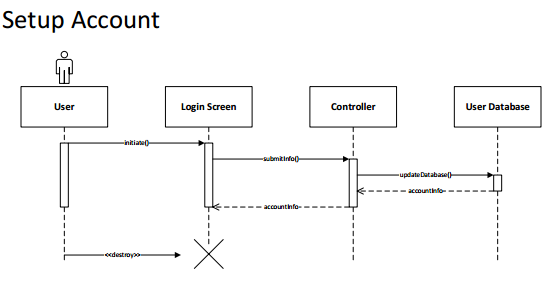
\includegraphics[scale=1]{../resources/SequenceDiagrams/setupAccount.png}\\
\includegraphics*[scale=1]{../resources/SequenceDiagrams/checkHistory.png}\\
\includegraphics*[scale=0.8]{../resources/SequenceDiagrams/searchForRock.png}\\

\section{Detailed Class Diagram}
See below the detailed class diagram for the system.\\

\bigskip
\includegraphics*[scale=0.35]{../resources/DetailedClassDiagram.png}\\


\newpage
\appendix
\section{Division of Labour}
\begin{center}
\begin{tabular}[!htbp]{| p{6cm} | p{6cm} | p{4cm} |} \hline
	\textbf{Team Member}	&\textbf{Contribution} 						& \textbf{Signature}	\\ \hline
	~					&~										&				\\
	Genevieve			&Introduction								&				\\ \hline
	~					&~										&				\\
	Nick					&State Charts								&				\\ \hline
	~					&										&				\\
	Niko					&Sequence Diagrams						&				\\ \hline
	~					&										&				\\
	Sydney				&Sequence Diagrams						&				\\ \hline
	~					&										&				\\
	Eric					&Detailed Class Diagram						&				\\ \hline
\end{tabular}
\end{center}

\end{document}